\section{训练后期}
在训练进行约$100~h$后,Q表逐渐收敛,此时学习鼠行为模式能够适应规则鼠的变化。图\ref{figure_matureheatmap}为这一时期$1~min$内机器鼠运动区域热点及轨迹图,与前期相比,这一时期两者的运动区域显然更加一致,运动轨迹高度相似。
\begin{figure}[htbp]
  \vspace{13pt}
  \centering
  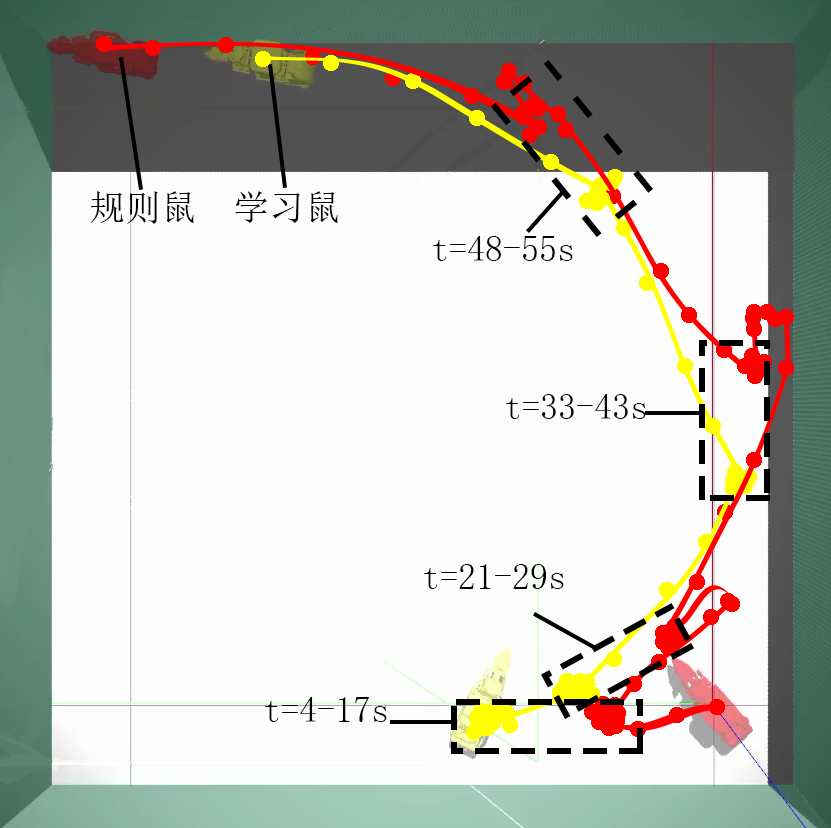
\includegraphics[height=6cm]{images/ch05/mature/heatmap.png}
  \caption{训练后期机器鼠运动热点图及运动轨迹($1~min$)}\label{figure_matureheatmap}
\end{figure} 

图\ref{figure_matureheatmap}展示了学习鼠具有跟随(follow)和接近(approach)交互对象的趋势,这也是生物鼠行为交互的重要模式之一。

从两者的距离上看(图\ref{figure_maturedistance}),学习鼠此时已经能够频繁进入规则鼠的有效交互距离以内,同时,当两者距离超出这一范围时,由于学习鼠训练得到的跟随特性,其能够迅速重新建立行为交互的联系。
\begin{figure}[htbp]
  \vspace{13pt}
  \centering
  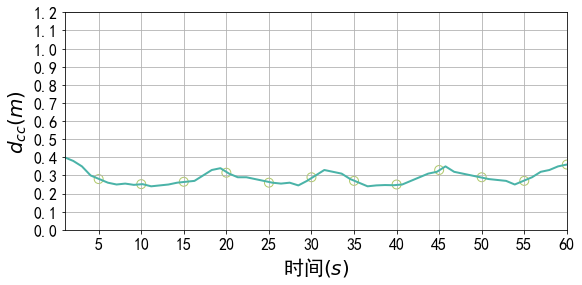
\includegraphics[height=6cm]{images/ch05/mature/distance.png}
  \caption{训练后期机器鼠中心距离($1~min$)}\label{figure_maturedistance}
\end{figure}

对生物鼠视频录像进行相同处理,得到在实验环境中观察到正在交互的两只生物鼠的活动区域热点图和活动轨迹如图\ref{figure_livingheatmap}。
\begin{figure}[htbp]
  \vspace{13pt}
  \centering
  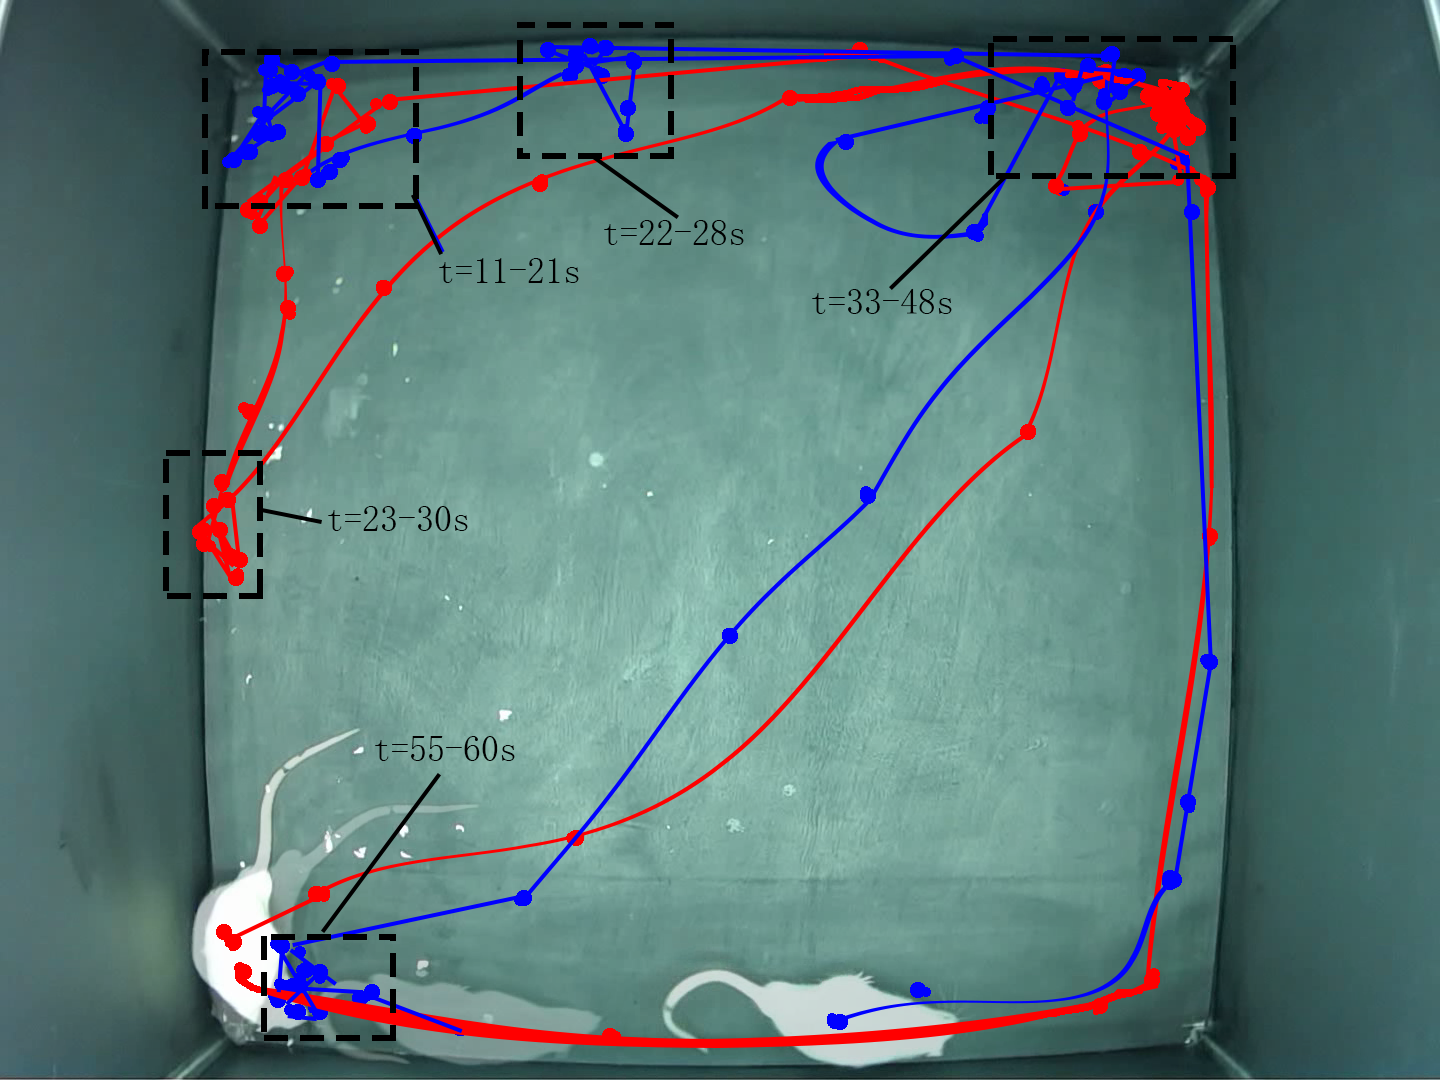
\includegraphics[height=6cm]{images/ch05/mature/livingheatmap.png}
  \caption{生物鼠运动热点图及运动轨迹($1~min$)}\label{figure_livingheatmap}
\end{figure} 

比较图\ref{figure_matureheatmap}和图\ref{figure_livingheatmap},可以发现经过Q-学习训练成熟的机器鼠在行为模式上与生物鼠具有一定的相似性,即均倾向于接近和跟随交互伙伴。但在运动范围和运动距离上,机器鼠的表现与生物鼠存在差异。图\ref{figure_livingdistance}展示了生物鼠中心距离$d_{cc}$的变化情况,与机器鼠相比,生物鼠的运动更加活跃,且$d_{cc}$的范围更广(最大超过$1~m$,最小仅为$0.06~m$)。造成这种差异的原因是由于Q-学习目标的单一性(本文设定学习鼠训练目标为与规则鼠开展有效交互),学习鼠必须时刻靠近规则鼠。同时由于状态划分以$d_{cc}=0.3~m$为界限,使得学习鼠在进入这一范围后不再靠近规则鼠。
\begin{figure}[htbp]
  \vspace{13pt}
  \centering
  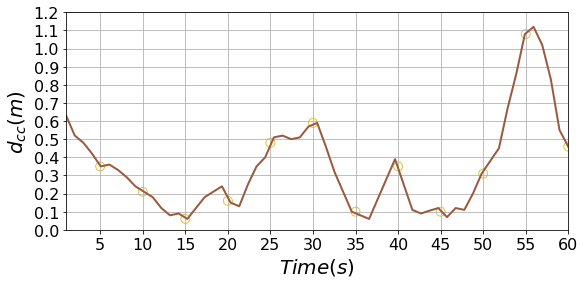
\includegraphics[height=6cm]{images/ch05/mature/livingdistance.png}
  \caption{生物鼠中心距离($1~min$)}\label{figure_livingdistance}
\end{figure}

图\ref{figure_matureheatmap}和图\ref{figure_livingheatmap}中都存在多处机器鼠或生物鼠停留较长的时段,在图\ref{figure_livingheatmap}中,这些时段意味着生物鼠进行了一些友好的交互行为(图\ref{figure_living15}、图\ref{figure_living37})。而在图\ref{figure_matureheatmap}中,机器鼠也产生了相似的行为(图\ref{figure_matureallow}、图\ref{figure_maturecon})。
\begin{figure}[htbp]
  \vspace{13pt}
  \centering
  \subfigure[$t=15~s$,征服]{\label{figure_living15}
  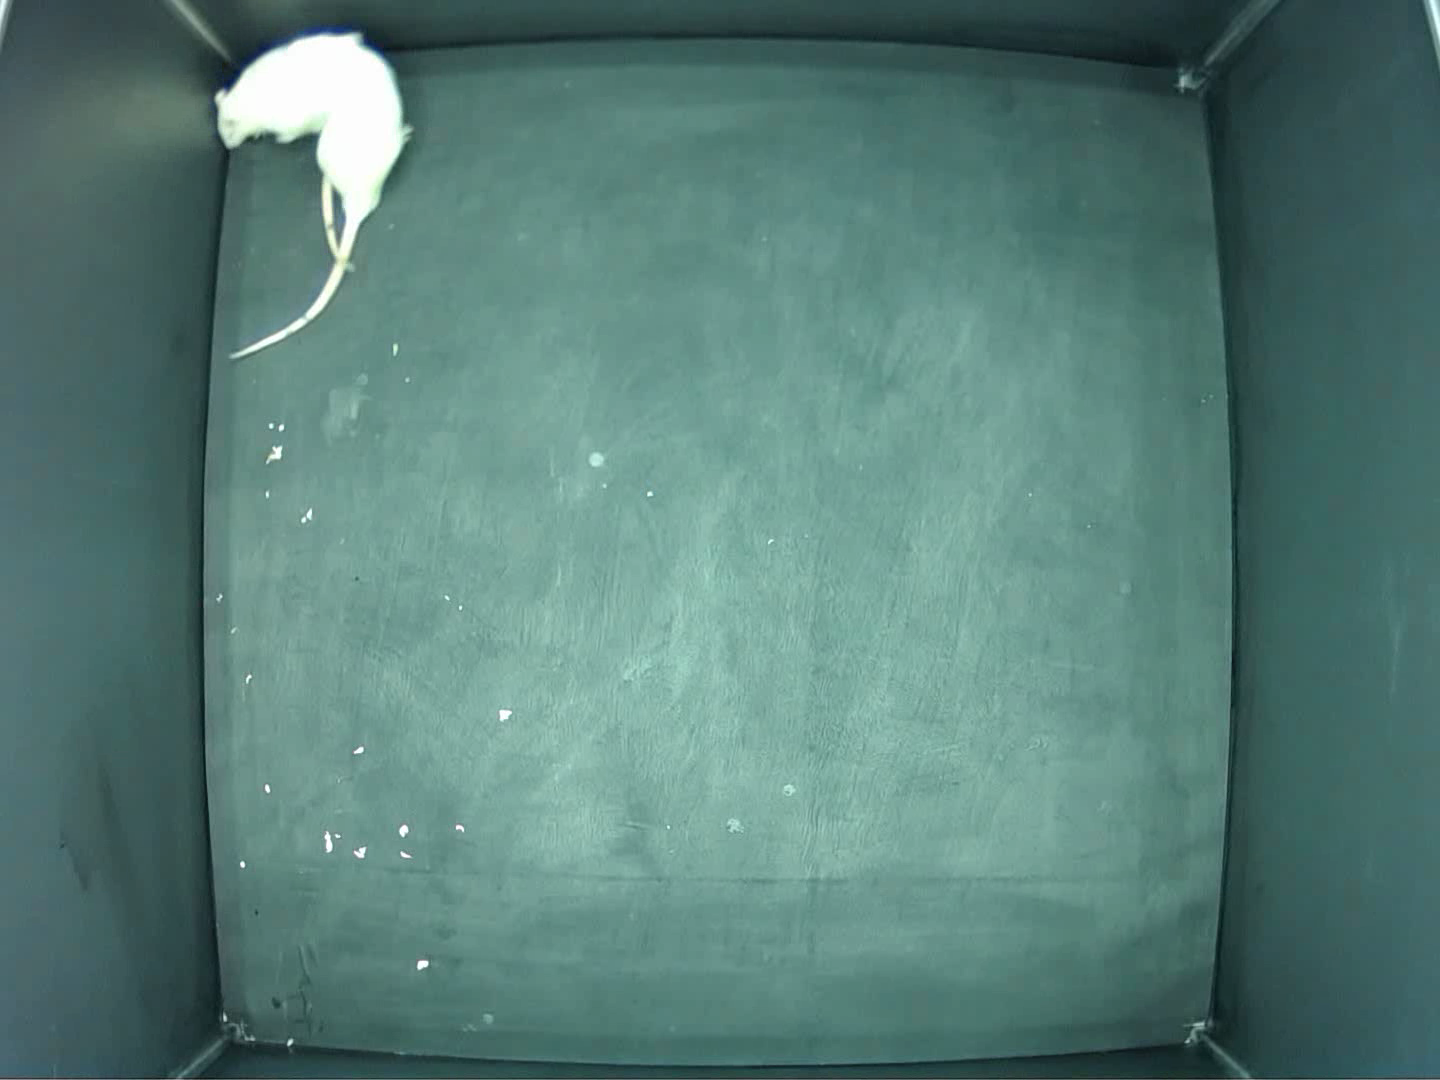
\includegraphics[height=2.5cm]{images/ch05/mature/living15.png}
  }
  \subfigure[$t=37~s$,嗅探]{\label{figure_living37}
  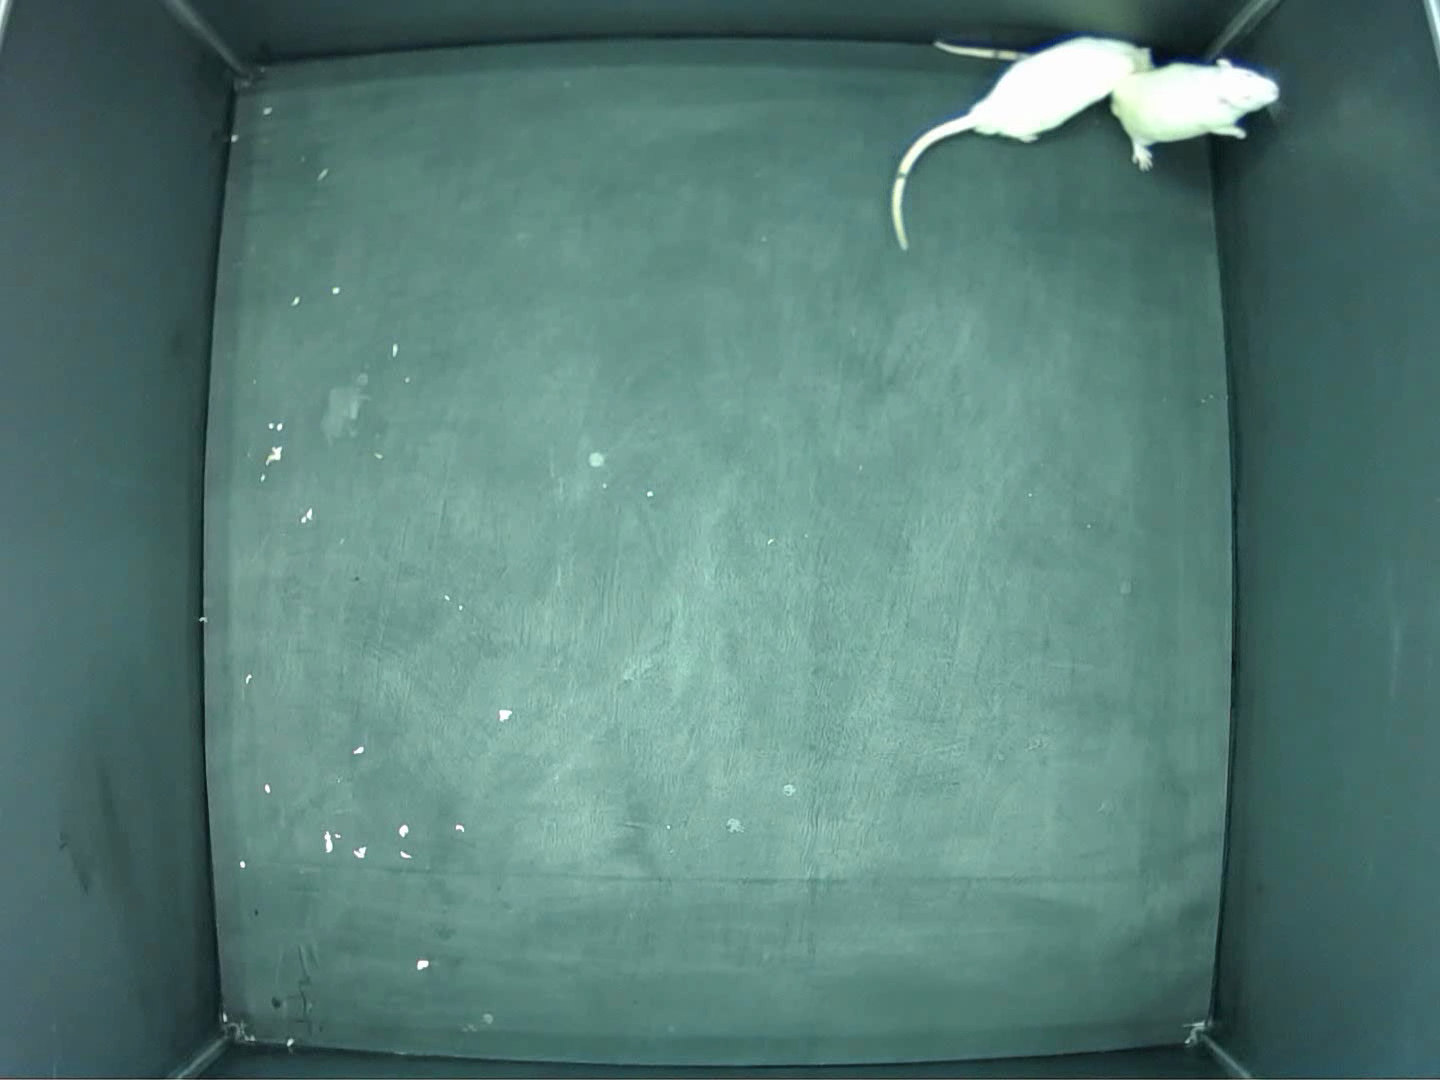
\includegraphics[height=2.5cm]{images/ch05/mature/living37.png}
  }
  \subfigure[$t=5~s$,梳理]{\label{figure_matureallow}
  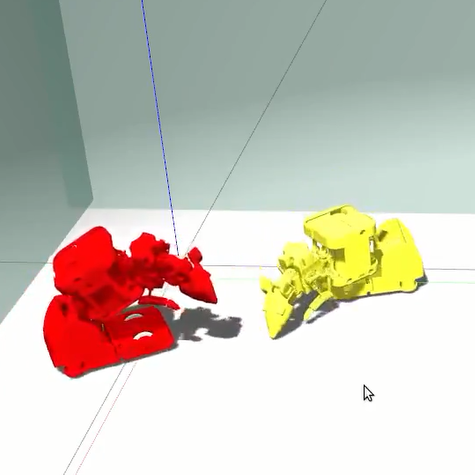
\includegraphics[height=2.5cm]{images/ch05/mature/allow.png}
  }
  \subfigure[$t=15~s$,征服]{\label{figure_maturecon}
  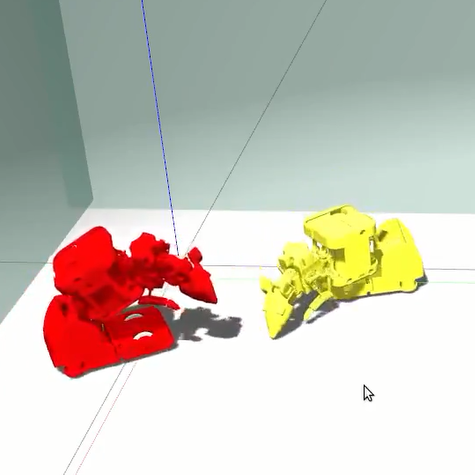
\includegraphics[height=2.5cm]{images/ch05/mature/allow.png}
  }
  \caption{生物鼠和机器鼠的一些友好交互行为}\label{figure_living1537}
\end{figure}

为考察机器鼠此阶段的整体交互性,尤其是当$d_{cc}<0.3~m$时的动作表现,将机器鼠每$1~s$内做出的主要动作进行统计,得到图\ref{figure_actionseq}。图中色条为对学习鼠和规则鼠该时刻产生动作的评价,评价越高则意味着此刻二者动作与生物鼠的行为交互相似度越高。
\begin{figure}[htb]
  \vspace{13pt}
  \centering
  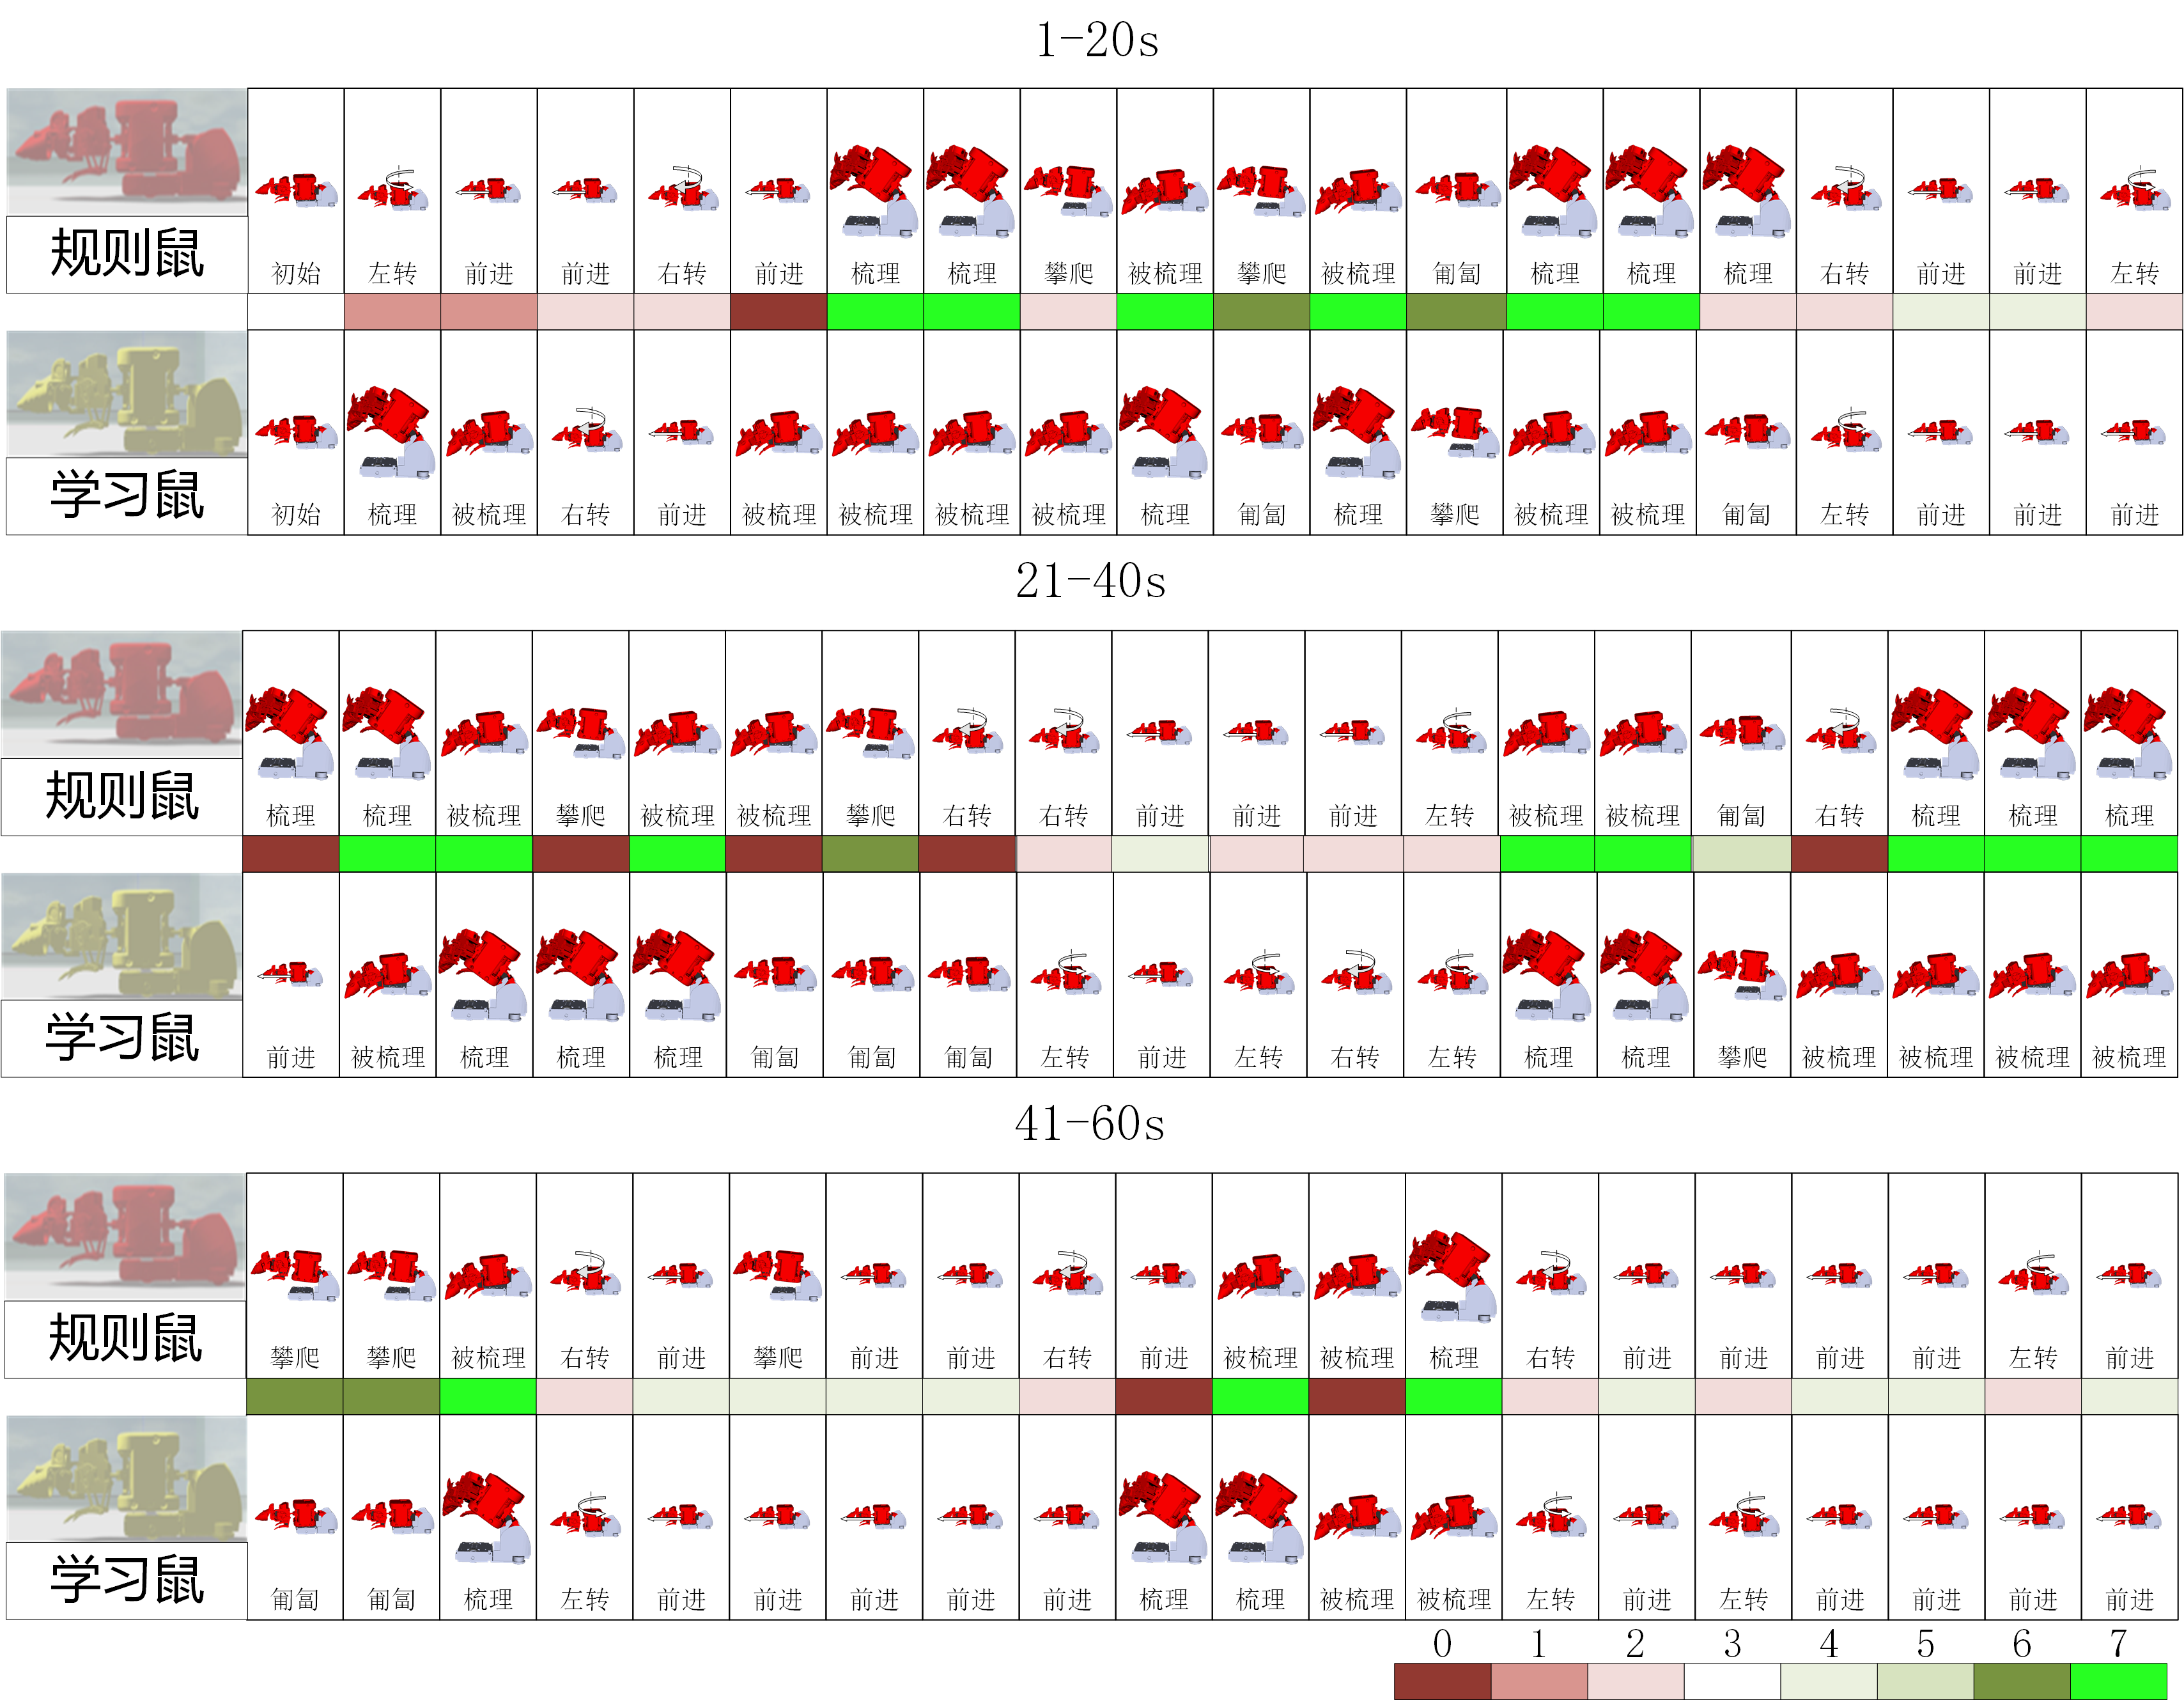
\includegraphics[width=1\linewidth]{images/ch05/mature/actionseq.png}
  \caption{机器鼠动作序列($1~min$)}\label{figure_actionseq}
\end{figure}

图\ref{figure_actionseq}显示,尽管在仿真中机器鼠出现表现不协调的时刻(评分为0),但这些时刻出现的频率较低(约为$13\%$),并且能够被迅速纠正(图中评分为0的时刻之后往往评分最高)。而具有较高相似度的动作持续时间一般较长,不易终止。表明这一阶段的学习鼠能够及时根据规则鼠的动作调整自身的动作,并且能以合适的方式引发规则鼠的交互行为。